\documentclass[hidelinks,12pt]{article}

\usepackage{amsmath, amsthm, amssymb, amsfonts}
\usepackage{thmtools}
\usepackage{graphicx}
\usepackage{setspace}
\usepackage{geometry}
\usepackage{float}
\usepackage{hyperref}
\usepackage[utf8]{inputenc}
\usepackage[english]{babel}
\usepackage{framed}
\usepackage[dvipsnames]{xcolor}
\usepackage[most]{tcolorbox}
\usepackage{parskip} % This package adjusts paragraph spacing properly

\setlength{\parindent}{0pt} % Removes the paragraph indent
\setlength{\parskip}{1em} % Adds vertical space between paragraphs

% The parskip package already sets the parskip to a non-zero value.


\tcbset{
    frame code={}
    center title,
    left=0pt,
    right=0pt,
    top=0pt,
    bottom=0pt,
    colback=gray!70,
    colframe=white,
    width=\dimexpr\textwidth\relax,
    enlarge left by=0mm,
    boxsep=5pt,
    arc=0pt,outer arc=0pt,
    }


\colorlet{LightGray}{White!90!Periwinkle}
\colorlet{LightOrange}{Orange!15}
\colorlet{LightGreen}{Green!15}

\newcommand{\HRule}[1]{\rule{\linewidth}{#1}}

\declaretheoremstyle[name=Theorem,]{thmsty}
\declaretheorem[style=thmsty,numberwithin=section]{theorem}
\tcolorboxenvironment{theorem}{colback=LightGray}

\declaretheoremstyle[name=Proposition,]{prosty}
\declaretheorem[style=prosty,numberlike=theorem]{proposition}
\tcolorboxenvironment{proposition}{colback=LightOrange}

\declaretheoremstyle[name=Principle,]{prcpsty}
\declaretheorem[style=prcpsty,numberlike=theorem]{principle}
\tcolorboxenvironment{principle}{colback=LightGreen}

\setstretch{1.2}
\geometry{
    textheight=9in,
    textwidth=5.5in,
    top=1in,
    headheight=12pt,
    headsep=25pt,
    footskip=30pt
}

% ------------------------------------------------------------------------------

\begin{document}

% ------------------------------------------------------------------------------
% Cover Page and ToC
% ------------------------------------------------------------------------------

\title{ \normalsize \textsc{}
		\\ [2.0cm]
		\HRule{1.5pt} \\
		\LARGE \textbf{\uppercase{Automata theory}
		\HRule{2.0pt} \\ [0.6cm] \LARGE{Exam materials} \vspace*{10\baselineskip}}
		}
\date{}
\author{\textbf{Author} \\ 
		Automata guy (AKA. Graph enjoyer) \\
		}

\maketitle
\newpage

\tableofcontents
\newpage

% ------------------------------------------------------------------------------

% \section{Examples}
%
% \begin{theorem}
%     This is a theorem.
% \end{theorem}
%
% \begin{proposition}
%     This is a proposition.
% \end{proposition}
%
% \begin{principle}
%     This is a principle.
% \end{principle}
%
% \subsection{Pictures}
%
% \begin{figure}[htbp]
%     \center
%     \includegraphics[scale=0.06]{img/photo.jpg}
%     \caption{Sydney, NSW}
% \end{figure}
%
% \subsection{Citation}
%
% This is a citation\cite{Eg}.
%
% \newpage

% ------------------------------------------------------------------------------
% Reference and Cited Works
% ------------------------------------------------------------------------------

% \bibliographystyle{IEEEtran}
% \bibliography{References.bib}

% ------------------------------------------------------------------------------


\section{Basic definitions}


\subsection{String}

A string is a finite sequence, possibly empty, of symbols drawn from some
alphabet $\Sigma$. Given any alphabet $\Sigma$, the shortest string that can be formed from $\Sigma$
is the empty string, which we will write as $\epsilon$. The set of all possible strings
over an alphabet $\Sigma$ is written $\Sigma$*. This notation exploits the Kleene star
operator, which we will define more generally below.

\subsection{Language}

A language is a (finite or infinite) set of strings over a finite alphabet $\Sigma$.
When we are talking about more than one language, we will use the notation $\Sigma_L$
to mean the alphabet from which the strings in the language L are formed.


\subsection{Alphabet}
An alphabet, denoted as $\Sigma$, is a non-empty finite set of symbols. These
symbols are the basic units used to construct strings. For example, $\Sigma =
\{a, b, c\}$ is an alphabet consisting of the symbols 'a', 'b', and 'c'.

\subsection{Kleene Star}
The Kleene star, denoted as $\Sigma^*$, is the set of all strings of finite
length that can be constructed from the alphabet $\Sigma$. This includes the
empty string $\epsilon$, as well as all possible concatenations of symbols from
$\Sigma$.

\subsection{Concatenation}
Concatenation is an operation that links two strings end to end. For strings
$x$ and $y$, the concatenation is denoted $xy$. If $L_1$ and $L_2$ are
languages, their concatenation is $L_1L_2 = \{xy | x \in L_1 \text{ and } y \in
L_2\}$.

\subsection{Substrings, Prefixes, and Suffixes}
A substring of a string is any sequence of consecutive symbols from that
string. A prefix is a substring that includes the first symbol of the string,
and a suffix is a substring that includes the last symbol of the string. For a
string $s$, a substring $t$ is such that $s = xty$ for some strings $x$ and
$y$.

\subsection{Reversal}
The reversal of a string $s$, denoted as $s^R$, is a string formed by writing
the symbols of $s$ in reverse order. For example, if $s = "abc"$, then $s^R =
"cba"$.


\subsection{Language Operations}
The union of languages $L_1$ and $L_2$, denoted by $L_1 \cup L_2$, is the set
of strings that are in either $L_1$ or $L_2$ or both. The intersection, denoted
by $L_1 \cap L_2$, is the set of strings that are in both $L_1$ and $L_2$. The
difference, denoted by $L_1 - L_2$, is the set of strings that are in $L_1$ but
not in $L_2$. The complement of a language $L$, denoted by $\overline{L}$, is
the set of all strings over $\Sigma$ that are not in $L$.

\subsection{Deterministic and Nondeterministic Machines}
Deterministic machines are computational models where for every state and
input, there is exactly one transition to a subsequent state. Nondeterministic
machines can have multiple possible transitions for a state and input pair.

\subsection{Transition Function}
The transition function of an automaton is a mapping from the cross product of
the state set and the input alphabet (including $\epsilon$ for nondeterministic
automata) to the power set of the state set. It defines the state transitions
of the automaton.

\subsection{Acceptance of a String}
A string $s$ over an alphabet $\Sigma$ is said to be accepted by an automaton
if, starting from the initial state and processing the symbols of $s$, the
automaton enters a final or accepting state after reading the entire string.

\subsection{Finite Automata}
Finite automata are abstract computational models that consist of states,
transitions between these states, and rules for starting and accepting inputs.
They are used to recognize regular languages.


\section{Finite state machines (FSM)}

\subsection{Acceptor}

Formally, a deterministic FSM (or DFSM) M is a quintuple $(K, \Sigma, , s, A)$,
where: 



\begin{itemize} 
\item $K$ is a finite set of states,
\item $\Sigma$ is the input alphabet, 
\item $s \in K$ is the start state, 
\item $A \subseteq K$ is the set of accepting states, and 
\item $\sigma$ is the transition function. It maps from:

		\begin{align*} K &\times \Sigma \to K \\ \end{align*}

\end{itemize}

A configuration of a DFSM M is an element of $K \times \Sigma$*. Think of it as a snapshot
of $M$. It captures the two things that can make a difference to $M$’s future
behavior:
\begin{itemize}
		\item its current state 
		\item the input that is still left to read.
\end{itemize}
M halts whenever it enters either an accepting or a rejecting configuration. It
will do so immediately after reading the last character of its input.

The language accepted by $M$, denoted $L(M)$, is the set of all strings accepted by
$M$.

\subsection{Equivalence of states}

\begin{enumerate}
		\item Acceptor states $q$ and $q'$ are not equivalent if exactly one of
		they have an accepting;

		\item Transformer states $q$ and $q'$ are not equivalent if any inputs
		for letter x print different letters $y \ne y'$;

		\item The states $q$ and $q'$ of any automaton are not equivalent if any
		for $x$ leads to nonequivalent states $f(q,x) \ne f(q',x)$;

		\item Otherwise, states $q$ and $q'$ are equivalent: $q \ne q'$.
\end{enumerate}

\subsection{Building DFA from NFA}

The algorithm will be shown with an example. We will need the $eps$ function.

$eps(q: state)$ =
\begin{enumerate}
		\item $result = {q}$.
		\item While there exists some $p \in result$ and some $r \in result$ and some transition $(p, \epsilon, r) \in \delta$ do:
		Insert r into result.
		\item Return $result$.
\end{enumerate}

\subsubsection{Example: Computing $eps$}

Consider the following NDFSM $M$:

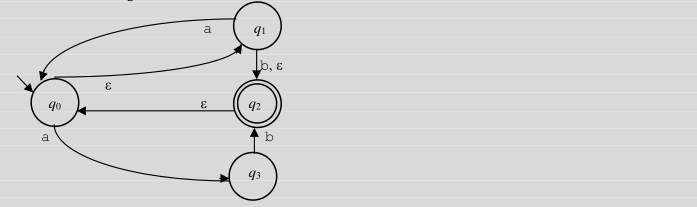
\includegraphics[width=\linewidth]{./img/eps.png}

To compute $eps(q_0)$, we initially set result to $\{q_0\}$. Then $q_1$ is added, producing $\{q_0, q_1\}$. Then $q_2$ is added, producing
$\{q_0, q_1, q_2\}$. There is an $\epsilon$-transition from $q_2$ to $q_0$, but $q_0$ is already in result. So the computation of $e(q_0)$ halts.
The result of running eps on each of the states of $M$ is:
\begin{align*}
		eps(q_0)&= \{q_0, q_1, q_2\}.\\
		eps(q_1)&= \{q_0, q_1, q_2\}.\\
		eps(q_2)&= \{q_0, q_1, q_2\}.\\
		eps(q_3)&= \{q_3\}.\\
\end{align*}

\subsubsection{Example: Building DFA from NFA}

Consider the following NDFSM $M$:

First, to get a feel for $M$, simulate it on the input string bbbacb, using coins
to keep track of the states it enters.



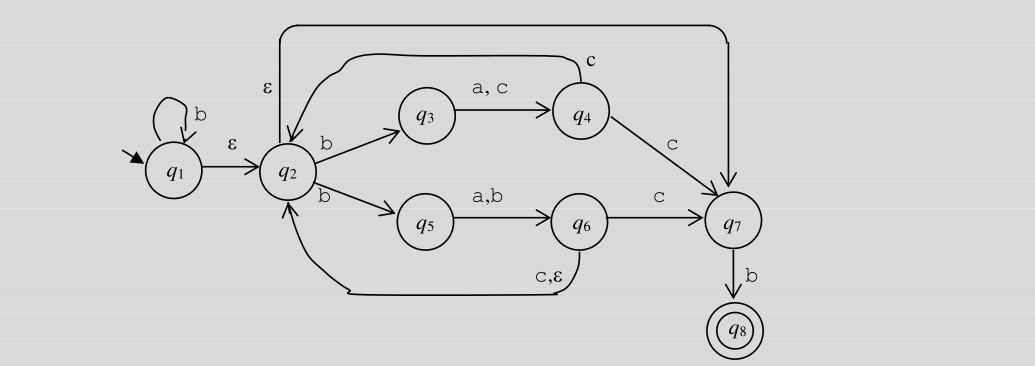
\includegraphics[width=\linewidth]{./img/ndfsmtodfsm1.png}

We can apply \texttt{ndfsmtodfsm} to \( M \) as follows:
\begin{enumerate}
    \item Compute \( \varepsilon(q) \) for each state \( q \) in \( K_M \):
    $ \varepsilon(q_1) = \{q_1, q_2, q_7\}, $
    $ \varepsilon(q_2) = \{q_2, q_7\}, $
    $ \varepsilon(q_3) = \{q_3\}, \varepsilon(q_4) = \{q_4\}, $
    $ \varepsilon(q_5) = \{q_5\}, $
    $ \varepsilon(q_6) = \{q_2, q_6, q_7\}, $
    $ \varepsilon(q_7) = \{q_7\}, \varepsilon(q_8) = \{q_8\}. $

    \item \( s' = \varepsilon(s) = \{q_1, q_2, q_7\} \).

    \item Compute \( \delta' \):
    $ \text{active-states} = \{\{q_1, q_2, q_7\}\}. 

		\text{ Consider } \{q_1, q_2, q_7\}: $
    $ ((\{q_1, q_2, q_7\}, a), \emptyset). $
    $ ((\{q_1, q_2, q_7\}, b), \{q_1, q_2, q_3, q_5, q_7, q_8\}). $
    $ ((\{q_1, q_2, q_7\}, c), \emptyset). $

    $ \text{active-states} = \{\{q_1, q_2, q_7\}, \emptyset, \{q_1, q_2, q_3, q_5, q_7, q_8\}\}. 

				\text{ Consider } \emptyset: $
    $ ((\emptyset, a), \emptyset). $
    $ /* \emptyset \text{ is a dead state and we will generally omit it.} $
    $ ((\emptyset, b), \emptyset). $
    $ ((\emptyset, c), \emptyset). $

    $ \text{active-states} = \{\{q_1, q_2, q_7\}, \emptyset, \{q_1, q_2, q_3, q_5, q_7, q_8\}, \{q_2, q_4, q_6, q_7\}, $
    $ \{q_1, q_2, q_3, q_5, q_6, q_7, q_8\}, \{q_4\}\}.$ 

		$\text{ Consider } \{q_2, q_4, q_6, q_7\}: $
    $ ((\{q_2, q_4, q_6, q_7\}, a), \emptyset). $
    $ ((\{q_2, q_4, q_6, q_7\}, b), \{q_3, q_5, q_8\}). $
    $ ((\{q_2, q_4, q_6, q_7\}, c), \{q_2, q_7\}). $

    $ \text{active-states} = \{\{q_1, q_2, q_7\}, \emptyset, \{q_1, q_2, q_3, q_5, q_7, q_8\}, \{q_2, q_4, q_6, q_7\}, $
    $ \{q_1, q_2, q_3, q_5, q_6, q_7, q_8\}, \{q_4\}, \{q_3, q_5, q_8\}, $
    $ \{q_2, q_7\}\}.$

				$ \text{ Consider } \{q_1, q_2, q_3, q_5, q_6, q_7, q_8\}: $
    $ ((\{q_1, q_2, q_3, q_5, q_6, q_7, q_8\}, a), \{q_2, q_4, q_6, q_7\}). $
    $ ((\{q_1, q_2, q_3, q_5, q_6, q_7, q_8\}, b), \{q_1, q_2, q_3, q_5, q_6, q_7, q_8\}). $
    $ ((\{q_1, q_2, q_3, q_5, q_6, q_7, q_8\}, c), \{q_2, q_4, q_7\}). $

    $ \text{active-states} = \{\{q_1, q_2, q_7\}, \emptyset, \{q_1, q_2, q_3, q_5, q_7, q_8\}, \{q_2, q_4, q_6, q_7\}, $
    $ \{q_1, q_2, q_3, q_5, q_6, q_7, q_8\}, \{q_4\}, \{q_3, q_5, q_8\}, $
    $ \{q_2, q_7\}, \{q_2, q_4, q_7\}\}.$

				$ \text{ Consider } \{q_4\}: $
    $ ((\{q_4\}, a), \emptyset). $
    $ ((\{q_4\}, b), \emptyset). $
    $ ((\{q_4\}, c), \{q_2, q_7\}). $

				\text{active-states did not change.} 

				\text{Consider} $ \{q_3, q_5, q_8\}:$
    $ ((\{q_3, q_5, q_8\}, a), \{q_2, q_4, q_6, q_7\}). $
    $ ((\{q_3, q_5, q_8\}, b), \{q_2, q_6, q_7\}). $
    $ ((\{q_3, q_5, q_8\}, c), \{q_4\}). $

    $ \text{active-states} = \{\{q_1, q_2, q_7\}, \emptyset, \{q_1, q_2, q_3, q_5, q_7, q_8\}, \{q_2, q_4, q_6, q_7\}, $
    $ \{q_1, q_2, q_3, q_5, q_6, q_7, q_8\}, \{q_4\}, \{q_3, q_5, q_8\}, $
    $ \{q_2, q_7\}, \{q_2, q_4, q_7\}, \{q_2, q_6, q_7\}\}.$ 

		\text{ Consider } \{q_2, q_7\}: $
    $ ((\{q_2, q_7\}, a), \emptyset). $
    $ ((\{q_2, q_7\}, b), \{q_3, q_5, q_8\}). $
    $ ((\{q_2, q_7\}, c), \emptyset). $

		\text{active-states did not change.} 

				\text{ Consider } \{q_2, q_4, q_7\}:
    $ ((\{q_2, q_4, q_7\}, a), \emptyset). $
    $ ((\{q_2, q_4, q_7\}, b), \{q_3, q_5, q_8\}). $
    $ ((\{q_2, q_4, q_7\}, c), \{q_2, q_7\}). $

    \text{active-states did not change. }

    \text{Consider } \{q_2, q_6, q_7\}:
    $ ((\{q_2, q_6, q_7\}, a), \emptyset). $
    $ ((\{q_2, q_6, q_7\}, b), \{q_3, q_5, q_8\}). $
    $ ((\{q_2, q_6, q_7\}, c), \{q_2, q_7\}). $

    \text{active-states did not change. } \delta' \text{ has been computed for each element of active-states.}
\end{enumerate}

\subsection{Transducer (Transformator)}

This definition for a deterministic finite state transducer permits each
machine to output any finite sequence of symbols as it makes each transition
(in other words, as it reads each symbol of its input).  FSMs that associate
outputs with transitions are called Mealy machines, after their inventor George
Mealy.  A Mealy machine $M$ is a six-tuple $(K, \Sigma, O, \delta, s, A)$, where: 

\begin{itemize}
	\item $K$ is a finite set of states,
	\item $\Sigma$ is an input alphabet,
	\item $O$ is an output alphabet,
	\item $s \in K$ is the start state,
	\item $A \subseteq K $ is the set of accepting states (although for some applications this designation is not important),
	\item $\sigma$ is the transition function. It is function $(K \times \Sigma) \to (K)$, and
	\item $D$ is the display or output function. It is a function from $(K) \to (O^*)$.
\end{itemize}

A Mealy (transducer defined above) machine $M$ computes a function $f(w)$ $
iff$, when it reads the input string $w$, its output sequence is $f(w)$. 

\subsubsection{Note on determinism}

Transducers are a class of automata used to model systems that transform input
sequences into output sequences. Moore and Mealy machines are two types of
transducers commonly studied in automata theory.

Both Moore and Mealy machines are inherently deterministic. In a deterministic
transducer:

\begin{itemize}
  \item Each state transition is uniquely determined by the current state and input symbol. The transition function $\delta$ of a Moore or Mealy machine maps each pair of current state and input symbol to exactly one next state.
  \item In the case of Moore machines, the output function $\lambda$ maps each state to exactly one output symbol, whereas in Mealy machines, the output function $\omega$ maps each pair of current state and input symbol to exactly one output symbol.
\end{itemize}

Determinism ensures that for any given input sequence, the transducer will
always produce the same output sequence and end in the same final state,
providing predictability and repeatability, which are essential properties for
many practical applications.
The concept of nondeterminism can be extended to transducers; however, this is not standard in classical automata.

\subsection{Probabalistic automata}

Probabalistic automata is defined by 6-tuple $(Q,X,p,q_A, q_0, \lambda)$:

\begin{itemize}
	\item $Q$ – set of states
	\item $X$ – input alphabet
	\item $p$ – transition function: $Q \times X \times Q → [0;1]$ or $X \to {[0;1]}^{|Q|\times|Q|}$
	\item $Q_A \subseteq Q$ – accepting states
	\item $q_0$ – initial state (sometimes $q0 \in [0;1]^{|Q|}$)
	\item $\lambda \in [0;1]$ – acceptance threshold (sometimes there is no $\lambda$) 
\end{itemize}

\subsubsection{Finding Accepting Words in Probabilistic Automata}

To determine whether a word is accepted by a probabilistic automaton, we
compute the probability of reaching an accepting state after processing the
word. The process involves two key steps:

\begin{enumerate}
  \item   For each word in the input alphabet, calculate the probability of transitioning from one state to another. This is done by summing up the probabilities of all possible paths that lead to an accepting state after processing the word. The transition function $p$ gives the probability of transitioning from one state to another given an input symbol.

  \item   Compare the calculated probability with the acceptance threshold $\lambda$. If the cumulative probability of reaching an accepting state is greater than or equal to $\lambda$, the word is accepted; otherwise, it is rejected.

\end{enumerate}

\subsubsection{Using Matrix Multiplication for Each Input}
Matrix multiplication can be used to efficiently compute the probabilities of transitioning between states for a given input string. Consider the transition matrix $P(x)$ for an input symbol $x \in X$, where each entry $P(x)_{ij}$ represents the probability of transitioning from state $i$ to state $j$ given the input $x$. The process is as follows:

\begin{enumerate}
  \item  Start with a row vector $\mathbf{v}$ representing the initial state distribution. If the initial state is certain, $\mathbf{v}$ is a one-hot vector with a 1 at the position corresponding to the initial state $q_0$.

  \item  For each symbol $x$ in the input string, multiply the current state vector $\mathbf{v}$ by the transition matrix $P(x)$. This results in a new state vector representing the probability distribution over states after processing $x$.

  \begin{align*}
		  \mathbf{v}' &= \mathbf{v} \cdot P(x)
  \end{align*}

  \item  After processing the entire input string, the final state vector $\mathbf{v}'$ gives the probability distribution over all states. The probability of being in an accepting state is the sum of the probabilities in $\mathbf{v}'$ corresponding to the accepting states.

\end{enumerate}


\subsection{Pumping lemma for Regular Languages }

\textbf{Theorem:} If $L$ is a regular language, then: 

\begin{align*}
		\exists k \ge 1 ( \forall \>\text{strings} \> w \in L, where |w| \ge k (x, y, z (w = &xyz, \\
		 |xy| &\le k, \\
		 y &\ne \epsilon, \text{and} \\
		\forallq &\ge 0 (xy^{q}z \in L)))). \\
\end{align*}
 
The Pumping Theorem tells us something that is true of every regular language.
Generally, if we already know that a language is regular, we won’t particularly
care about what the Pumping Theorem tells us about it. But suppose that we are
interested in some language $L$ and we want to know whether or not it is
regular. If we could show that the claims made in the Pumping Theorem are not
true of $L$, then we would know that $L$ is not regular. It is in arguments
such as this that we will find the Pumping Theorem very useful. In particular,
we will use it to construct proofs by contradiction. We will say, “If $L$ were
regular, then it would possess certain properties. But it does not possess
those properties. Therefore, it is not regular.”

To make maximum use of the Pumping Theorem’s requirement that $y$ fall in the
first $k$ characters, it is often a good idea to choose a string $w$ that is
substantially longer than the $k$ characters required by the theorem. In
particular, if $w$ can be chosen so that there is a uniform first region of
length at least $k$, it may be possible to consider just a single case for
where $y$ can fall. The Pumping Theorem inspires poets, as we’ll see in Chapter
10. $A^nB^n$ is a simple language that illustrates the kind of property that
characterizes languages that aren’t regular. It isn’t of much practical
importance, but it is typical of a family of languages, many of which are of
more practical significance. In the next example, we consider $Bal$, the
language of balanced parentheses. The structure of $Bal$ is very similar to
that of $A^nB^n$. $Bal$ is important because most languages for describing
arithmetic expressions, Boolean queries, and markup systems require balanced
delimiters.

\subsubsection{Example: Even Palindrome Language is Not Regular}

The Even Palindrome Language is Not Regular Let $L$ be $PalEven = \{ww : w \in
\{a, b\}^*\}$. $PalEven$ is the language of even-length palindromes of a’s and
b’s. We can use the Pumping Theorem to show that $PalEven$ is not regular. If
it were, then there would exist some $k$ such that any string $w$, where $|w|
\geq k$, must satisfy the conditions of the theorem. We show one string $w$
that does not. (Note here that the variable $w$ used in the definition of $L$
is different from the variable $w$ mentioned in the Pumping Theorem.) We will
choose $w$ so that we only have to consider one case for where $y$ could fall.
Let $w = a^kb^kb^ka^k$. Since $|w| = 4k$ and $w$ is in $L$, $w$ must satisfy
the conditions of the Pumping Theorem. So there must exist $x, y,$ and $z$,
such that $w = xyz$, $|xy| \leq k$, $y \neq \epsilon$, and $\forall q \geq 0
(xy^qz \in L)$. Since $|xy| \leq k$, $y$ must occur within the first $k$
characters and so $y = a^p$ for some $p$. Since $y \neq \epsilon$, $p$ must be
greater than $0$. Let $q = 2$. The resulting string is $a^{k+p}b^kb^ka^k$. If
$p$ is odd, then this string is not in $PalEven$ because all strings in
$PalEven$ have even length. If $p$ is even then it is at least $2$, so the
first half of the string has more a’s than the second half does, so it is not
in $PalEven$. So $L = PalEven$ is not regular.

\subsubsection{Example: $A^nB^n$ Language is Not Regular }

$A^nB^n$ is not Regular. Let $L$ be $A^nB^n = \{a^nb^n : n \neq 0\}$. We can
use the Pumping Theorem to show that $L$ is not regular. If it were, then there
would exist some $k$ such that any string $w$, where $|w| \geq k$, must satisfy
the conditions of the theorem. We show one string $w$ that does not. Let $w =
a^kb^k$. Since $|w| = 2k$, and $w$ is in $L$, it must satisfy the conditions of
the Pumping Theorem. Therefore, there must exist $x, y,$ and $z$ such that $w =
xyz$, $|xy| \leq k$, $y \neq \epsilon$, and $\forall q \geq 0 (xy^qz \in L)$.
Since $|xy| \leq k$, $y$ must occur within the first $k$ characters and
therefore $y = a^p$ for some $p$. Since $y \neq \epsilon$, $p$ must be greater
than $0$. Let $q = 2$. The resulting string is $a^{k+p}b^k$. The last condition
of the Pumping Theorem states that this string must be in $L$, but it is not,
since it has more $a$’s than $b$’s. Thus, there exists at least one long string
in $L$ that fails to satisfy the conditions of the Pumping Theorem. Therefore,
$L = A^nB^n$ is not regular.


\section{Regex (Regular expressions)}

A regular expression over an alphabet $\Sigma$ is a formal way of representing
a regular language. It is constructed from members of $\Sigma$ using union
(denoted by $+$), concatenation, Kleene star, and parentheses for grouping.

A regular expression is a string that can be formed according to the following rules:
\begin{enumerate}
	\item $\emptyset$ is a regular expression.
	\item $\epsilon$ is a regular expression.
	\item Every element in $\Sigma$ is a regular expression.
	\item Given two regular expressions $\alpha$ and $\beta$, $\alpha\beta$ is a regular expression.
	\item Given two regular expressions $\alpha$ and $\beta$, $\alpha \lor \beta$ is a regular expression.
	\item Given a regular expression $\alpha$, $\alpha^*$ is a regular expression.
	\item Given a regular expression $\alpha$, $\alpha^+$ is a regular expression.
	\item Given a regular expression $\alpha$, ($\alpha$) is a regular expression.
\end{enumerate}

Define the following semantic interpretation function \( L \) for the language of regular expressions:

\begin{enumerate}
    \item \( L(\emptyset) = \emptyset \), the language that contains no strings.
    \item \( L(\epsilon) = \{\epsilon\} \), the language that contains just the empty string.
    \item For any \( c \in \Sigma \), \( L(c) = \{c\} \), the language that contains the single, one-character string \( c \).
    \item For any regular expressions \( \alpha \) and \( \beta \), \( L(\alpha \beta) = L(\alpha) L(\beta) \). In other words, to form the meaning of the concatenation of two regular expressions, first determine the meaning of each of the constituents. Both meanings will be languages. Then concatenate the two languages together. Recall that the concatenation of two languages \( L_1 \) and \( L_2 \) is \( \{ w = xy \mid x \in L_1 \text{ and } y \in L_2 \} \). Note that, if either \( L(\alpha) \) or \( L(\beta) \) is equal to \( \emptyset \), then the concatenation will also be equal to \( \emptyset \).
    \item For any regular expressions \( \alpha \) and \( \beta \), \( L(\alpha \cup \beta) = L(\alpha) \cup L(\beta) \). Again we form the meaning of the larger expression by first determining the meaning of each of the constituents. Each of them is a language. The meaning of \( \alpha \cup \beta \) then, as suggested by our choice of the character \( \cup \) as an operator, is the union of the two constituent languages.
    \item For any regular expression \( \alpha \), \( L(\alpha^*) = (L(\alpha))^* \), where \( * \) is the Kleene star operator defined in Section 2.2.5. So \( L(\alpha^*) \) is the language that is formed by concatenating together zero or more strings drawn from \( L(\alpha) \).
    \item For any regular expression \( \alpha \), \( L(\alpha^+) = L(\alpha \alpha^*) = L(\alpha) (L(\alpha))^* \). If \( L(\alpha) \) is equal to \( \emptyset \), then \( L(\alpha^+) \) is also equal to \( \emptyset \). Otherwise \( L(\alpha^+) \) is the language that is formed by concatenating together one or more strings drawn from \( L(\alpha) \).
    \item For any regular expression \( \alpha \), \( L((\alpha)) = L(\alpha) \). In other words, parentheses have no effect on meaning except to group the constituents in an expression.
\end{enumerate}


\begin{itemize}
		\item * asterisk indicates zero or more occurrences of the preceding element.
		For example, ab*c matches "ac", "abc", "abbc", "abbbc", and so on. 

		\item + the plus sign indicates one or more occurrences of the preceding element.
		For example, ab+c matches "abc", "abbc", "abbbc", and so on, but not "ac". 
\end{itemize}


\subsection{Building Regex from FSM}


\begin{itemize}

\item If $\alpha$ is the regular expression $\beta \cup \gamma$ and if both $L(\beta)$ and $L(\gamma)$ are regular,
then we construct $M_3 = (K_3, \Sigma, \Delta_3, s_3, A_3)$ such that $L(M_3) = L(\alpha) = L(\beta) \cup L(\gamma)$. If necessary, rename the states of $M_1$ and $M_2$ so that $K_1  K_2 = $. Create
a new start state, $s_3$, and connect it to the start states of $M_1$ and $M_2$ via
$\epsilon$-transitions. $M_3$ accepts if either $M_1$ or $M_2$ accepts. So $M_3 = ({s_3} \cup K_1 \cup K_2, \Sigma, \Delta_3, s_3, A_1 \cup A_2)$, where $\Delta3 = \Delta1 \cup \Delta2 \cup {((s_3, \epsilon), s_1), ((s_3, \epsilon), s_2)}$.

\item If $\alpha$ is the regular expression $\beta\gamma$ and if both $L(\beta)$ and $L(\gamma)$ are regular, then
we construct $M_3 = (K_3, \Sigma, \Delta_3, s_3, A_3)$ such that $L(M_3) = L(\alpha) = L(\beta) L(\gamma)$. If
necessary, rename the states of $M_1$ and $M_2$ so that $K_1 \cap K_2 = \emptyset$. We will build $M_3$
by connecting every accepting state of $M_1$ to the start state of $M_2$ via an
$\epsilon$-transition. $M_3$ will start in the start state of $M_1$ and will accept if $M_2$
does. So $M_3 = (K_1 \cup K_2, \Sigma, \Delta_3, s_1, A_2)$, where $\Delta_3 = \Delta_1 \cup \Delta_2 \cup \{((q, \epsilon), s_2) : q
\in A_1\}$.

\item If $\alpha$ is the regular expression $\beta^*$ and if $L(\beta)$ is regular, then we construct
$M_2 = (K_2, \Sigma, \Delta_2, s_2, A_2)$ such that $L(M_2) = L(\alpha) = L(\beta)^*$. We will create a new
start state $s_2$ and make it accepting, thus assuring that $M_2$ accepts $\epsilon$. (We need
a new start state because it is possible that $s_1$, the start state of $M_1$, is not
an accepting state. If it isn't and if it is reachable via any input string
other than $\epsilon$, then simply making it an accepting state would cause $M_2$ to accept
strings that are not in $(L(M_1))^*$.) We link the new $s_2$ to $s_1$ via an
$\epsilon$-transition. Finally, we create $\epsilon$-transitions from each of $M_1$’s accepting
states back to $s_1$. So $M_2 = (\{s_2\} \cup K_1, \Sigma, \Delta_2, s_2, \{s_2\} \cup A_1)$, where $\Delta_2 = \Delta_1 \cup
\{((s_2, \epsilon), s_1)\} \cup \{((q, \epsilon), s_1) : q \in A_1\}$. 

\end{itemize}

Notice that the machines that these constructions build are typically highly
nondeterministic because of their use of $\epsilon$-transitions. They also typically
have a large number of unnecessary states. But, as a practical matter, that is
not a problem since, given an arbitrary NDFSM $M$, we have an algorithm that can
construct an equivalent DFSM $M'$. We also have an algorithm that can minimize $M'$.

\subsubsection{Example: Building FSM from Regex}

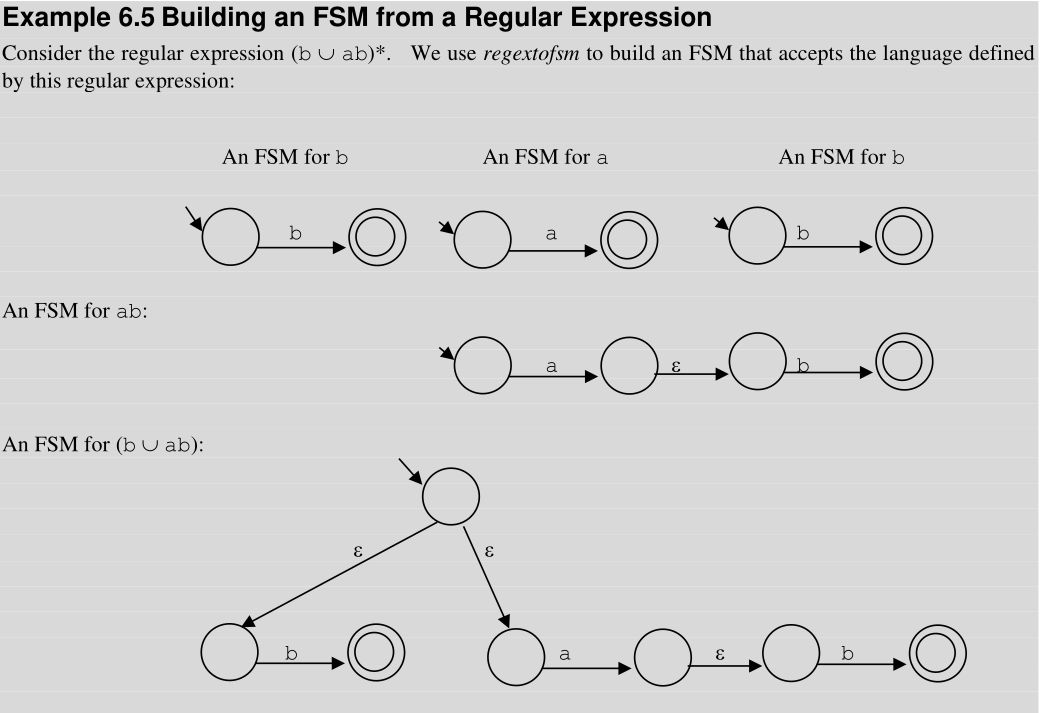
\includegraphics[width=\textwidth]{img/regextofsm1.png}
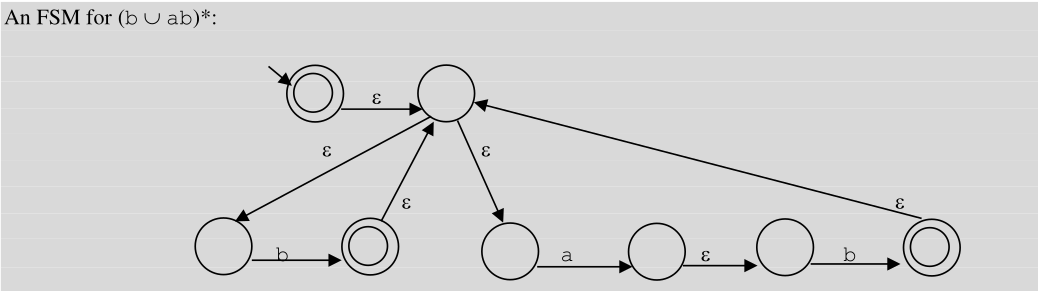
\includegraphics[width=\textwidth]{img/regextofsm2.png}

\subsection{Building Regex from FSM}

Next we must show how to build FSMs to accept languages that are defined by
regular expressions that exploit the operations of concatenation, union, and
Kleene star. Let $\beta$ and $\gamma$ be regular expressions that define
languages over the alphabet $\Sigma$. If $L(\beta)$ is regular, then it is
accepted by some FSM $M_1 = (K_1, \Sigma, \Delta_1, s_1, A_1)$. If $L(\gamma)$
is regular, then it is accepted by some $FSM M_2 = (K_2, \Sigma, \Delta_2, s_2,
A_2)$.

fsmtoregexheuristic(M: FSM) =
\begin{enumerate}
  \item Remove from $M$ any states that are unreachable from the start state.

  \item If $M$ has no accepting states then halt and return the simple
  regular expression $\emptyset$.
  
  \item If the start state of $M$ is part of a loop (i.e., it has any
  transitions coming into it), create a new start state $s$
  and connect $s$ to $M$’s start state via an
  $\epsilon$-transition. This new start state $s$ will have
  no transitions into it.
  
  \item If there is more than one accepting state of $M$ or if there is
		  just one but there are any transitions out of it,
		  create a new accepting state and connect each
		  of $M$’s accepting states to it via an
		  $\epsilon$-transition. Remove the old accepting states
		  from the set of accepting states. Note that the
		  new accepting state will have no transitions
		  out from it.
\end{enumerate}

\subsubsection{Example: Building Regex from FSM}


%     \includegraphics[scale=0.06]{img/photo.jpg}
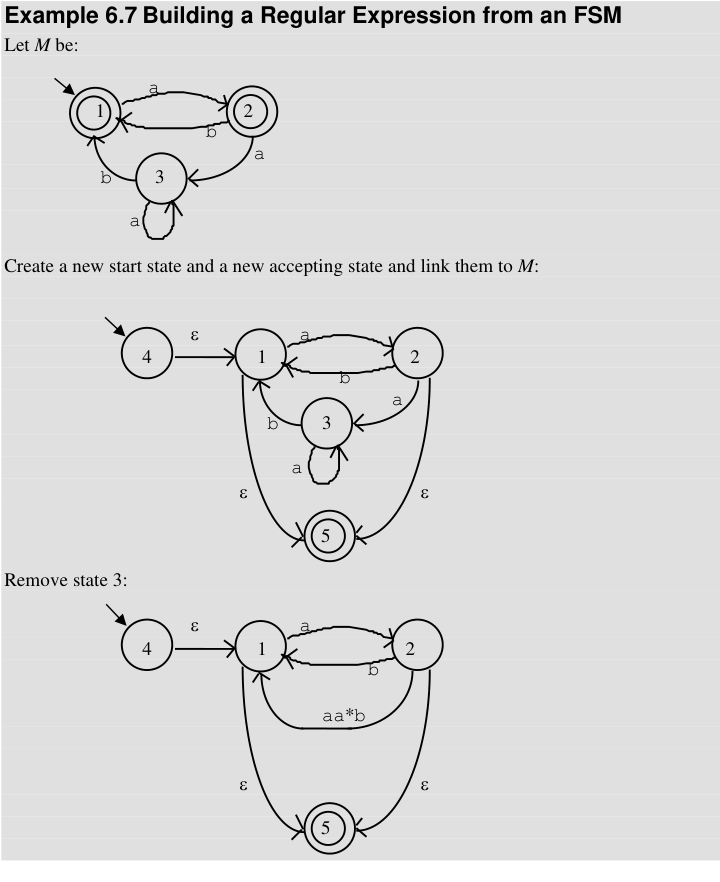
\includegraphics[width=\textwidth]{img/fsmtoregex1.png}
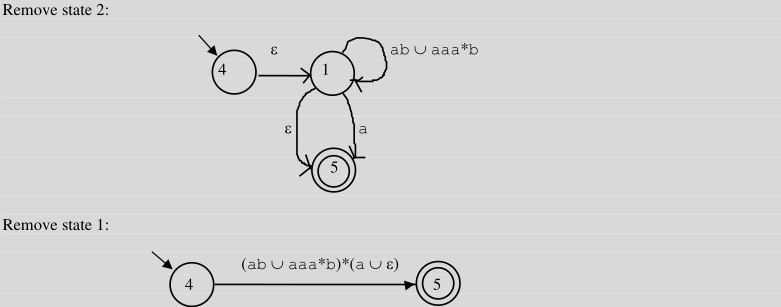
\includegraphics[width=\textwidth]{img/fsmtoregex2.png}

\section{PDA (Pushdown automata)}

\subsection{Definition of a (Nondeterministic) PDA }

A pushdown automaton, or PDA, is a finite state machine that has been augmented
by a single stack. In a minute, we will present the formal definition of the
PDA model that we will use. But, before we do that, one caveat to readers of
other books is in order. There are several competing PDA definitions, from
which we have chosen one to present here. All are provably equivalent, in the
sense that, for all $i$ and $j$, if there exists a version$i$ PDA that accepts
some language $L$ then there also exists a version$j$ PDA that accepts $L$.
We’ll return to this issue in Section 12.5, where we will mention a few of the
other models and sketch an equivalence proof. For now, simply beware of the
fact that other definitions are also in widespread use.


We will use the following definition: A pushdown automaton (or PDA) $M$ is a
six-tuple $(K, \Sigma, \Gamma, \Delta, s, A)$, where:
 
\begin{itemize}
	\item $K$ is a finite set of states, 
	\item $\Sigma$ is the input alphabet, 
	\item $\Sum$ is the stack alphabet, 
	\item $s \in K$ is the start state, 
	\item $A \subseteq K$ K is the set of accepting states, and 
	\item $\Delta$ is the transition relation.  It is a finite subset of  
\begin{align*}
\left(
		\left( K \times (\Sigma \cup \{\epsilon\}) \times \Gamma  \right) \times \left( K \times \Gamma^*  \right)
\right)
\end{align*}
\end{itemize}

We will use the following notational convention for describing $M$’s stack as a
string: The top of the stack is to the left of the string.

If a $c_1c_2\ldots c_n$ of characters is pushed onto the stack, they
will be pushed rightmost first, so if the value of the stack before the push
was $s$, the value after the push will be $c_1c_2\ldots c_ns$.

Note two things about what a transition $((q_1, c_1, c_2), (q_2, \gamma))$
says about how $M$ manipulates its stack:

\begin{itemize}
  \item $M$ may only take the transition if the character $c_2$ matches the current top of the stack. If it does, and the transition is taken, then $M$ pops $c_2$ and then pushes $\gamma$. $M$ cannot “peek” at the top of its stack without popping off the values that it examines.
  \item If $c_2 = \epsilon$, then $M$ must match $\epsilon$ against the top of the stack. But $\epsilon$ matches everywhere. So letting $\gamma$ be $\epsilon$ is equivalent to saying “without bothering to check the current value of the stack”. It is not equivalent to saying, “if the stack is empty.” In our definition, there is no way to say that directly, although we will see that we can create a way by letting $M$, before it does anything else, push a special marker onto the stack. Then, whenever that marker is on the top of the stack, the stack is otherwise empty.
\end{itemize}

$C$ is an accepting computation iff $C = (s, w, \alpha)|-_{M}^{*}(q, \epsilon, \beta)$, for some $q \in A$. 
In our definition there are no restrictions on final stack contents. In other words, PDA accepts
if it reaches the accepting configuration with no regard to the stack contents.

\end{document}
